\documentclass[12pt,xcolor={dvipsnames}]{beamer}

\mode<trans>{
\usepackage{pgfpages}
\pgfpagesuselayout{4 on 1}[a4paper,border shrink=2mm,landscape]
}

\usetheme[
%%% option passed to the outer theme
%    progressstyle=fixedCircCnt,   % fixedCircCnt, movingCircCnt (moving is deault)
  ]{Feather}

% If you want to change the colors of the various elements in the theme, edit and uncomment the following lines

\graphicspath {{images/}}

% Change the bar colors:
\setbeamercolor{Feather}{fg=Mahogany!20,bg=Mahogany}

% Change the color of the structural elements:
\setbeamercolor{structure}{fg=Sepia}

% Change the frame title text color:
\setbeamercolor{frametitle}{fg=black!5}

% Change the normal text colors:
\setbeamercolor{normal text}{fg=black!75,bg=gray!5}

%% Change the block title colors
\setbeamercolor{block title}{use=Feather,bg=Feather.fg, fg=black!90}


% Change the logo in the upper right circle:
%\renewcommand{\logofile}{example-grid-100x100pt}
%% This is an image that comes with the LaTeX installation
% Adjust scale of the logo w.r.t. the circle; default is 0.875
% \renewcommand{\logoscale}{0.55}

% Change the background image on the title and final page.
% It stretches to fill the entire frame!
\renewcommand{\backgroundfile}{pyds}%{numericalmethods_1}

%-------------------------------------------------------
% INCLUDE PACKAGES
%-------------------------------------------------------

\usepackage[utf8]{inputenc}
\usepackage[english]{babel}
\usepackage[T1]{fontenc}
%\usepackage{helvet}

%% Load different font packages to use different fonts
%% e.g. using Linux Libertine, Linux Biolinum and Inconsolata
%\usepackage{libertine}
%\usepackage{zi4}

\usepackage{multicol}

%% e.g. using Carlito and Caladea
\usepackage{carlito}
\usepackage{caladea}
\usepackage{zi4}

%% e.g. using Venturis ADF Serif and Sans
%\usepackage{venturis}

%-------------------------------------------------------
% DEFFINING AND REDEFINING COMMANDS
%-------------------------------------------------------

% colored hyperlinks
\newcommand{\chref}[2]{
  \href{#1}{{\usebeamercolor[bg]{Feather}#2}}
}

%-------------------------------------------------------
% INFORMATION IN THE TITLE PAGE
%-------------------------------------------------------

%\usepackage{pgf,pgfarrows,pgfnodes,pgfautomata,pgfheaps,pgfshade}
\usepackage{tikz}
\usepackage{amsmath,amssymb}
\usepackage{colortbl}
%\usepackage{times}
\usepackage{rotating}
\usepackage{multirow}
\usepackage{mathrsfs}
\usepackage{pgf}
\usepackage{media9}
\usepackage{listings}
\usepackage{hyperref}
\usepackage{longtable,booktabs}
\usepackage{upquote}
\usepackage{animate}

\definecolor{codegreen}{rgb}{0,0.6,0}
\definecolor{codegray}{rgb}{0.5,0.5,0.5}
\definecolor{codepurple}{rgb}{0.58,0,0.82}
\definecolor{backcolour}{rgb}{0.95,0.95,0.92}

\lstdefinestyle{mystyle}{
    backgroundcolor=\color{backcolour},
    commentstyle=\color{codegreen},
    keywordstyle=\color{magenta},
    numberstyle=\tiny\color{codegray},
    stringstyle=\color{codepurple},
    basicstyle=\ttfamily,
    breakatwhitespace=false,
    breaklines=true,
    captionpos=b,
    keepspaces=true,
    numbers=left,
    numbersep=5pt,
    showspaces=false,
    showstringspaces=false,
    showtabs=false,
    tabsize=2
}

\lstset{style=mystyle}

%%% For continuing the enumeration numbering in slides
\newcounter{saveenumi}
\newcommand{\seti}{\setcounter{saveenumi}{\value{enumi}}}
\newcommand{\conti}{\setcounter{enumi}{\value{saveenumi}}}
%%%%

\newtheorem{thm}{Thoerem}
\newtheorem{cor}{Corollary}
\newtheorem{lem}{Lemma}
\newtheorem{prop}{Proposition}
\newtheorem{defn}{Definition}
\newtheorem{rem}{Remark}
\newtheorem{prob}{Problem}
\newtheorem{prog}{Program}

\usetikzlibrary{arrows,shapes,backgrounds}
\hypersetup{pdfpagemode=FullScreen}
%\setbeamercovered{dynamic}

\tikzstyle{every picture}+=[remember picture]
\tikzstyle{na} = [baseline=-.5ex]

\renewcommand{\logofile}{VITEmblemLogo}
\renewcommand{\logoscale}{0.65}

%Emblem
%\pgfdeclareimage[height=1cm]{logo}{VITEmblemLogo}%{AUEmblem}

%\pgfdeclareimage[height=2cm]{logo}{Ashoka_Chakra_10} %%Uncoment this for India Flag Theme

\title[MAT6003 - Python Programming for Data Science]{{\textbf{MAT6003 - Programming for Data Science}}\\\textbf{Linear Regression using Scikit-Learn}}
\subtitle[]{Dr. B.S.R.V. Prasad\\srvprasad.bh@vit.ac.in}
%\author[Dr. B.S.R.V. Prasad]{\bf Dr. B.S.R.V. Prasad\\Department of Mathematics\\School of Advanced Sciences\\VIT, Vellore}
\date{}%{\small{\bf srvprasad.bh@gmail.com\\srvprasad.bh@vit.ac.in}}

%\logo{\pgfuseimage{logo}}

\begin{document}

{\1% % this is the name of the PDF file for the background
\begin{frame}[plain,noframenumbering] % the plain option removes the header from the title page, noframenumbering removes the numbering of this frame only
  \titlepage % call the title page information from above
\end{frame}}

\begin{frame}{Linear Regression using Scikit-Learn}
\begin{itemize}
\item In this tutorial, we study the most fundamental machine learning algorithms i.e., linear regression using Scikit-learn machine learning library.
\item We discuss the Python implementation of both simple linear regression and multiple linear regression.
\end{itemize}
\end{frame}

\begin{frame}{Linear Regression Theory - Review}
\begin{itemize}
\item Linear regression performs the task to predict a dependent variable
value ($y$) based on a given independent variable ($x$) using a linear relationship between $x$ and $y$.
\item If we plot the
independent variable ($x$) on the $x-$axis and dependent variable ($y$) on the
$y-$axis, linear regression gives us a straight line that best fits the
data points, as shown in the figure below.
\end{itemize}
\end{frame}

\begin{frame}{Liner Regression Theory - Review}
\begin{figure}
\centering
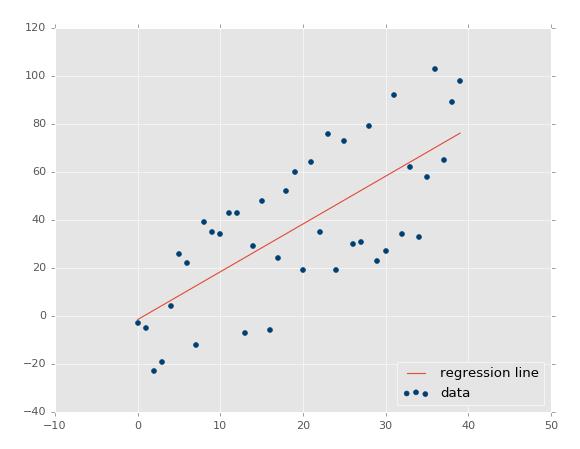
\includegraphics[scale=0.4]{LReg_1.png}
\end{figure}
\end{frame}

\begin{frame}[shrink=10]{Linear Regression Theory - Review}
The equation of the above line is :
$$ y= mx + b $$

\begin{quote}\small{
\begin{itemize}
\item Here, b is the intercept and m is the slope of the line.
\item Basically,
the linear regression algorithm gives us the most optimal value for the
intercept and the slope (in two dimensions).
\item The $y$ and $x$ variables
remain the same, since they are the data features and cannot be changed.
\item The values that we can control are the intercept($b$) and slope($m$).
\item There
can be multiple straight lines depending upon the values of intercept
and slope.
\item  Basically what the linear regression algorithm does is it
fits multiple lines on the data points and returns the line that results
in the least error.
\end{itemize}}
\end{quote}
\end{frame}

\begin{frame}{Liner Regression Theory - Review}
\begin{center}
\animategraphics[loop,autoplay,scale=0.4]{1.6}{LR_Re2-}{0}{14}
\end{center}
\end{frame}

\begin{frame}{Linear Regression Theory - Review}
\begin{itemize}
\item This same concept can be extended to cases where there are more than two
variables and is called multiple linear regression.
\begin{itemize}
\item For instance, consider a scenario where you have to predict the price of the house
based upon its area, number of bedrooms, the average income of the
people in the area, the age of the house, and so on.
\end{itemize}
\item In this case, the dependent variable (target variable) is dependent upon several
independent variables. A regression model involving multiple variables
can be represented as:
$$y = b_0 + m_1b_1 + m_2b_2 + m_3b_3 + \dotsc + m_nb_n$$
\end{itemize}
\end{frame}

\begin{frame}{Linear Regression Theory - Review}
\begin{itemize}
  \item The above equation is called \textbf{hyperplane}.
  \item Linear regression in two dimensions is a straight line; in three dimensions it is a plane; and in more than three dimensions, a hyperplane.
\end{itemize}
\end{frame}

\section{Simple Linear Regression}

\begin{frame}{Simple Linear Regression using Scikit-Learn}
For discussing the simple linear regression using Scikit-learn, we use the dataset on weather reports from the period of World war II to compare
with missions in the bombing operations dataset. This is a publicly available dataset and can be downloaded from \href{https://drive.google.com/open?id=1fiHg5DyvQeRC4SyhsVnje5dhJNyVWpO1}{\textbf{here}}\\\bigskip

The dataset contains information on weather conditions recorded on each day at various weather stations around the world. Information includes precipitation, snowfall, temperatures, wind speed and whether the day included thunderstorms or other poor weather conditions.\\\bigskip

Our task is to predict the maximum temperature taking input feature as the minimum temperature.
\end{frame}

\begin{frame}[fragile]{Simple Linear Regression using Scikit-Learn}
Import the required packages
\begin{lstlisting}[language=Python]
import pandas as pd
import numpy as np
import matplotlib.pyplot as plt
import seaborn as seabornInstance
from sklearn.model_selection import train_test_split
from sklearn.linear_model import LinearRegression
from sklearn import metrics
\end{lstlisting}
\end{frame}

\begin{frame}[fragile]{Simple Linear Regression using Scikit-Learn}
We now import the CSV dataset into a DataFrame using pandas:
\begin{lstlisting}[language=Python]
dataset = pd.read_csv('Weather.csv')
\end{lstlisting}
We now explore the dataset attributes and statistical description
\begin{lstlisting}[language=Python]
print('Dataset size is: ',dataset.shape)
print(dataset.describe())
\end{lstlisting}
\end{frame}

\begin{frame}{Simple Linear Regression using Scikit-Learn}
\begin{figure}
\centering
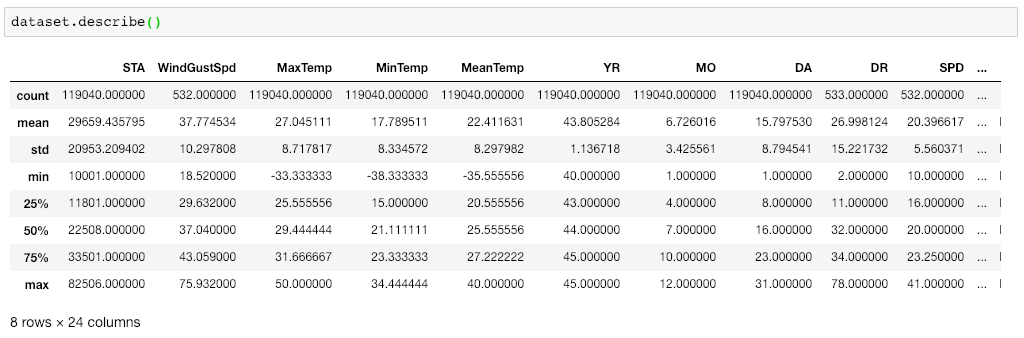
\includegraphics[scale=0.3]{LR_Reg3.png}
\end{figure}
\end{frame}

\begin{frame}[fragile]{Simple Linear Regression using Scikit-Learn}
Before proceeding to linear regression, first let's plot our data points related to MinTemp and MaxTemp on a $2-$D graph to view our
dataset and see if we can manually find any relationship between the data:
\begin{lstlisting}[language=Python]
dataset.plot(x='MinTemp', y='MaxTemp', style='o', figsize=(15,10))
plt.title('MinTemp vs MaxTemp')
plt.xlabel('MinTemp')
plt.ylabel('MaxTemp')
plt.show()
\end{lstlisting}
\end{frame}

\begin{frame}{Simple Linear Regression using Scikit-Learn}
\begin{figure}
\centering
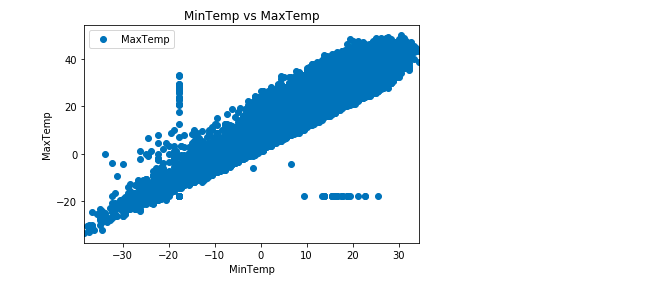
\includegraphics[scale=0.6]{LR_Reg4.png}
\end{figure}
\end{frame}

\begin{frame}[fragile]{Simple Linear Regression using Scikit-Learn}
We now plot Average Maximum Temperature along with univariate distribution of observations. For this we will use  \lstinline[language=Python]!seaborn.distplot()!
\begin{lstlisting}[language=Python]
plt.figure(figsize=(15,10))
plt.tight_layout()
seabornInstance.distplot(dataset['MaxTemp'])
\end{lstlisting}
\end{frame}

\begin{frame}{Simple Linear Regression using Scikit-Learn}
\begin{figure}
\centering
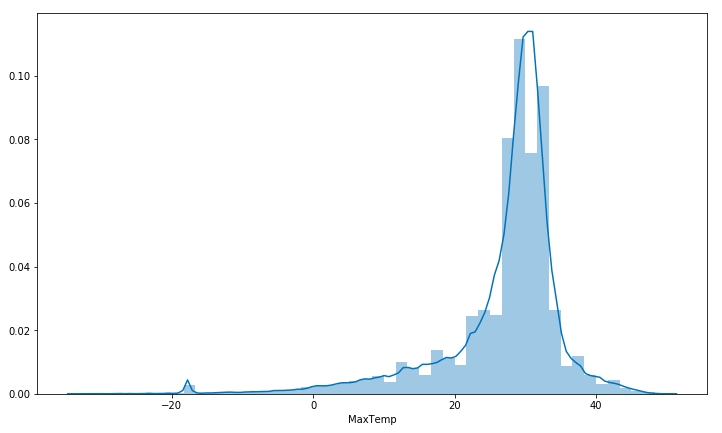
\includegraphics[scale=0.3]{LR_Reg5.png}
\end{figure}
Observe that Average Maximum temperature which is in between 25 and 35.
\end{frame}

\begin{frame}{Simple Linear Regression using Scikit-Learn}
\begin{itemize}
\item Our next step is to divide the data into ``\textbf{attributes}'' and ``\textbf{labels}''.
\item \textbf{Attributes} are the independent variables while \textbf{labels} are dependent
variables whose values are to be predicted.
\item In our dataset, we only have two columns.
\item We want to predict the MaxTemp depending upon the MinTemp
recorded.
\item Therefore our attribute set will consist of the ``MinTemp''
column which is stored in the X variable, and the label will be the
``MaxTemp'' column which is stored in y variable.
\end{itemize}
\end{frame}

\begin{frame}[fragile]{Simple Linear Regression using Scikit-Learn}
\begin{lstlisting}[language=Python]
X = dataset['MinTemp'].values.reshape(-1,1)
y = dataset['MaxTemp'].values.reshape(-1,1)

print('Attributes size is: ',X.shape)
print('Labels size is: ',y.shape)
\end{lstlisting}
\end{frame}

\begin{frame}{Simple Linear Regression using Scikit-Learn}
\begin{itemize}
\item Next, we split 80\% of the data to the training set while 20\% of the data to test set using \lstinline[language=Python]!tranin_test_split()! function of \lstinline[language=Python]!sklearn.model_selection!.
\item The test\_size variable is where we actually specify the proportion of the test set.
\end{itemize}
\end{frame}

\begin{frame}[fragile]{Simple Linear Regression using Scikit-Learn}
\begin{lstlisting}[language=Python]
X_train, X_test, y_train, y_test = train_test_split(X, y, test_size=0.2, random_state=0)

print('Training Attributes size is: ',X_train.shape)
print('Testing Attributes size is: ',X_test.shape)
print('Training Labels size is: ',y_train.shape)
print('Testing Lables size is: ' ,y_test.shape)
\end{lstlisting}
\end{frame}

\begin{frame}[fragile]{Simple Linear Regression using Scikit-Learn}
\begin{itemize}
\item After splitting the data into training and testing sets, finally, the time is to train our algorithm.
\item For that, we need to import \lstinline[language=Python]!LinearRegression! class, instantiate it, and call the \lstinline[language=Python]!fit()! method along with our training data.
\end{itemize}
\begin{lstlisting}[language=Python]
regressor = LinearRegression()
regressor.fit(X_train, y_train) #training the algorithm
\end{lstlisting}
\end{frame}

\begin{frame}[fragile,shrink=12]{Simple Linear Regression using Scikit-Learn}
\begin{itemize}
\item The linear regression model basically finds the best value for the intercept and slope, which results in a line that best fits the data.
\item To see the value of the intercept and slope calculated by the linear regression algorithm for our dataset, execute the following code.
\end{itemize}
\begin{lstlisting}[language=Python]
print('Intercept is: ',regressor.intercept_) #To retrieve the intercept:
print('Coefficient is: ',regressor.coef_) #For retrieving the slope:
\end{lstlisting}
Result is:
\begin{lstlisting}[language=Python]
10.66185201
0.92033997
\end{lstlisting}

\alert{This means that for every one unit of change in Min temperature, the change in the Max temperature is about 0.92\%.}
\end{frame}

\begin{frame}[fragile,shrink=5]{Simple Linear Regression using Scikit-Learn}
\begin{itemize}
\item Now that we have trained our algorithm, it’s time to make some predictions.
\item To do so, we will use our test data and see how accurately our algorithm predicts the percentage score.
\item To make predictions on the test data, execute the following code.
\end{itemize}
\begin{lstlisting}[language=Python]
y_pred = regressor.predict(X_test)
\end{lstlisting}
\begin{itemize}
\item Now compare the actual output values for `X\_test` with the predicted values.
\end{itemize}
\begin{lstlisting}[language=Python]
df = pd.DataFrame({'Actual': y_test.flatten(), 'Predicted': y_pred.flatten()})
df
\end{lstlisting}
\end{frame}

\begin{frame}{Simple Linear Regression using Scikit-Learn}
\begin{figure}
\centering
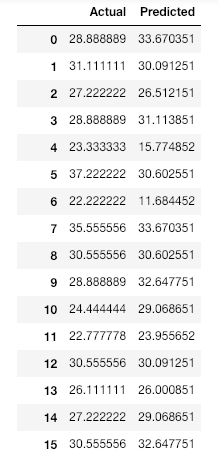
\includegraphics[scale=0.7]{LR_Reg6.png}
\end{figure}
\end{frame}

\begin{frame}[fragile]{Simple Linear Regression using Scikit-Learn}
\begin{itemize}
\item We can also visualize comparison result as a bar graph.\\ Note: As the number of records is huge, for representation purpose we will consider the first 25 records only.
\end{itemize}
\begin{lstlisting}[language=Python]
df1 = df.head(25)
df1.plot(kind='bar',figsize=(15,10))
plt.grid(which='major', linestyle='-', linewidth='0.5', color='green')
plt.grid(which='minor', linestyle=':', linewidth='0.5', color='black')
plt.show()
\end{lstlisting}
\end{frame}

\begin{frame}{Simple Linear Regression using Scikit-Learn}
\begin{figure}
\centering
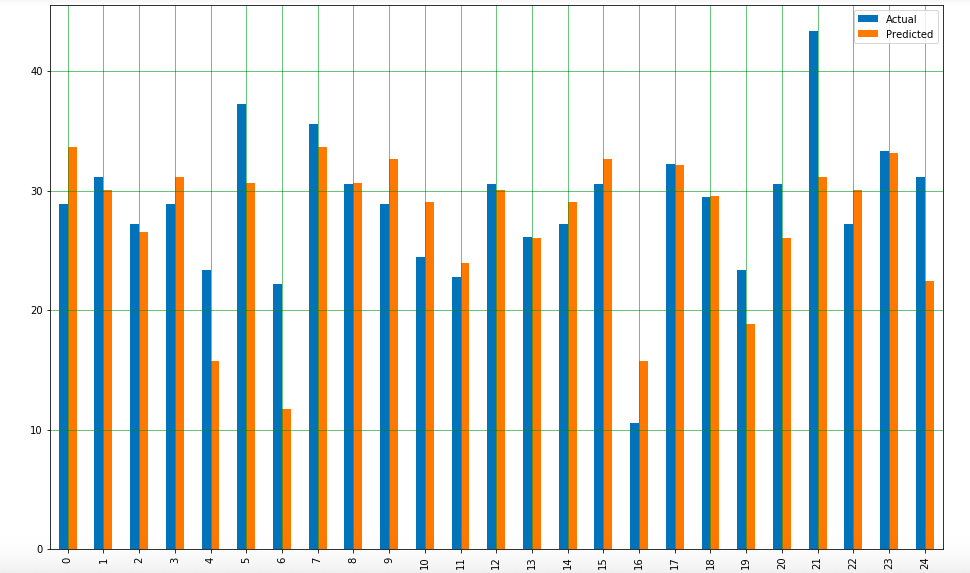
\includegraphics[scale=0.3]{LR_Reg7.png}
\end{figure}
\end{frame}

\begin{frame}[fragile]{Simple Linear Regression using Scikit-Learn}
\begin{itemize}
\item We now plot the straight line with the test data.
\end{itemize}
\begin{lstlisting}[language=Python]
plt.figure(figsize=(15,10))
plt.scatter(X_test, y_test,  color='gray')
plt.plot(X_test, y_pred, color='red', linewidth=2)
plt.show()
\end{lstlisting}
The straight line above shows that our algorithm is working correctly.
\end{frame}

\begin{frame}{Simple Linear Regression using Scikit-Learn}
\begin{itemize}
\item The final step in our modelling approach is to evaluate the performance of our algorithm.
\item This is very important step to compare how well different algorithms perform on a particular dataset.
\end{itemize}
\end{frame}

\begin{frame}[shrink=20]{Simple Linear Regression using Scikit-Learn}
\begin{itemize}
\item For regession algorithms, three evaluation metrics are commonly used:
\begin{description}
  \item[1. Mean Absolute Error (MAE)] is the mean of the absolute of the errors. It is calculated as:
  $$\text{MAE} = \frac{1}{n}\sum\limits_{i=1}^n \left|Y_i - y_i\right|$$
  \item[2. Mean Squared Error (MSE)] is the mean of the squared errors. It is calculated as:
  $$\text{MSE} = \frac{1}{n}\sum\limits_{i=1}^n \left(Y_i - y_i\right)^2$$
  \item[3. Root Mean Squared Error (RMSE)] is the square root of the mean of the squared errors. It is calculated as:
  $$\text{RMSE} = \sqrt{\frac{1}{n}\sum\limits_{i=1}^n \left(Y_i - y_i\right)^2}$$
\end{description}
\end{itemize}
\end{frame}

\begin{frame}[fragile]{Simple Linear Regression using Scikit-Learn}
\begin{itemize}
\item The above tree metrics can be computed using the pre-built functions in \lstinline[language=Python]!sklearn.metrics! library.
\end{itemize}
\begin{lstlisting}[language=Python]
print('Mean Absolute Error:', metrics.mean_absolute_error(y_test, y_pred))
print('Mean Squared Error:', metrics.mean_squared_error(y_test, y_pred))
print('Root Mean Squared Error:', np.sqrt(metrics.mean_squared_error(y_test, y_pred)))
\end{lstlisting}
\end{frame}

\begin{frame}[fragile]{Simple Linear Regression using Scikit-Learn}
Output:
\begin{lstlisting}[language=Python]
('Mean Absolute Error:', 3.19932917837853)
('Mean Squared Error:', 17.631568097568447)
('Root Mean Squared Error:', 4.198996082109204)
\end{lstlisting}
\begin{itemize}
\item Observe that the RMS error is $4.19$, which is more than $10\%$ of the mean value of the percentages of all the temperature i.e, $22.41$.
\item This means that our algorithm was not very accurate but can still make reasonably good predictions.
\end{itemize}
\end{frame}
\end{document}


